\documentclass[11pt]{article}
\usepackage[a4paper,margin=1in]{geometry}
\usepackage{hyperref}
\usepackage{graphicx}
\usepackage{xcolor}
\usepackage{listings}
\usepackage{longtable}
\usepackage{array}
\usepackage{enumitem}
\usepackage{booktabs}

\usepackage{tikz}
\usetikzlibrary{positioning,arrows.meta}

\hypersetup{
  colorlinks=true,
  linkcolor=blue,
  urlcolor=blue
}

\lstdefinelanguage{SQL}{
  keywords={
    SELECT,INSERT,UPDATE,DELETE,FROM,WHERE,JOIN,LEFT,RIGHT,INNER,OUTER,ON,CREATE,ALTER,DROP,PRIMARY,KEY,FOREIGN,REFERENCES,
    TABLE,VIEW,FUNCTION,RETURNS,LANGUAGE,BEGIN,END,DECLARE,IF,THEN,ELSE,CASE,WHEN,AS,AND,OR,NOT,IN,EXISTS,UNION,ALL,
    CHECK,CONSTRAINT,DEFAULT,RETURNING,WITH,SERIAL,INT,INTEGER,NUMERIC,TEXT,VARCHAR,JSONB,TIMESTAMP,CURRENT_TIMESTAMP,
    DISTINCT,TRUE,FALSE,RAISE,NOTICE,EXCEPTION,SET,VALUES,INTO,PERFORM,DO,GRANT,REVOKE,SCHEMA,EXTENSION
  },
  sensitive=false,
  comment=[l]--,
  morecomment=[s]{/*}{*/},
  morestring=[b]',
}
\lstset{
  language=SQL,
  basicstyle=\ttfamily\small,
  keywordstyle=\color{blue!70!black}\bfseries,
  commentstyle=\color{green!40!black},
  stringstyle=\color{red!60!black},
  numbers=left,
  numberstyle=\scriptsize\color{gray},
  stepnumber=1,
  numbersep=8pt,
  backgroundcolor=\color{gray!5},
  frame=single,
  breaklines=true,
  columns=fullflexible,
  showstringspaces=false,
  tabsize=2
}

\begin{document}

\begin{titlepage}
\centering
{\LARGE Database Design \& ETL Automation — Project Documentation\par}
\vspace{1em}
{\large \textbf{Students:} Oltean Simion, Ihos Iarina, Cuibus Dorin, Andreican Rares\quad \par}
\vfill
{\large \today\par}
\end{titlepage}


\section{Project Overview}
\textbf{Goal.} Build a fully automated pipeline that ingests a CSV dataset into a \emph{staging} area, then normalizes it into a \emph{production} schema using idempotent, scheduled ETL jobs.\\[2pt]
\textbf{Stack.} PostgreSQL 16, \texttt{pg\_cron}, Docker.\\[2pt]


\section{Dataset Summary}
The dataset (\texttt{dataset.csv}) models students and their academic-to-career journey. Fields used by the ETL are:

\begin{longtable}{>{\ttfamily}p{0.28\linewidth}p{0.64\linewidth}}
\toprule
student\_id & Natural key for a student (string, unique).\\
age & Student's age (integer).\\
gender & Gender label (string).\\
high\_school\_gpa & HS GPA in [2.00, 4.00].\\
sat\_score & SAT score in [900, 1600].\\
university\_gpa & University GPA in [2.00, 4.00].\\
field\_of\_study & Bachelor's major/field.\\
internships\_completed & 0--4.\\
projects\_completed & 0--9.\\
certifications & 0--5.\\
soft\_skills\_score & 1--10.\\
networking\_score & 1--10.\\
job\_offers & 0--5.\\
starting\_salary & 25{,}000--1{,}000{,}000.\\
career\_satisfaction & 1--10.\\
years\_to\_promotion & 1--5.\\
current\_job\_level & Entry/Mid/Senior/Executive.\\
work\_life\_balance & 1--10.\\
entrepreneurship & Yes/No.\\
\bottomrule
\end{longtable}

\section{Architecture \& Workflow}
\subsection*{High-level Flow}
\begin{enumerate}[leftmargin=1.5em]
  \item \textbf{Ingestion to Staging.} A scheduled job checks if \texttt{dataset.csv} changed (using file modification time) and \textbf{upserts} JSON rows into \texttt{staging.events}.
  \item \textbf{Transform/Load to Production.} Another scheduled job materializes the normalized model into four production tables with \texttt{INSERT \ldots ON CONFLICT DO UPDATE} (idempotent).
  \item \textbf{Logging.} All runs are captured in \texttt{etl\_logs.job\_runs} with status: \emph{running}, \emph{completed}, \emph{skipped}, or \emph{failed}.
\end{enumerate}

\begin{center}
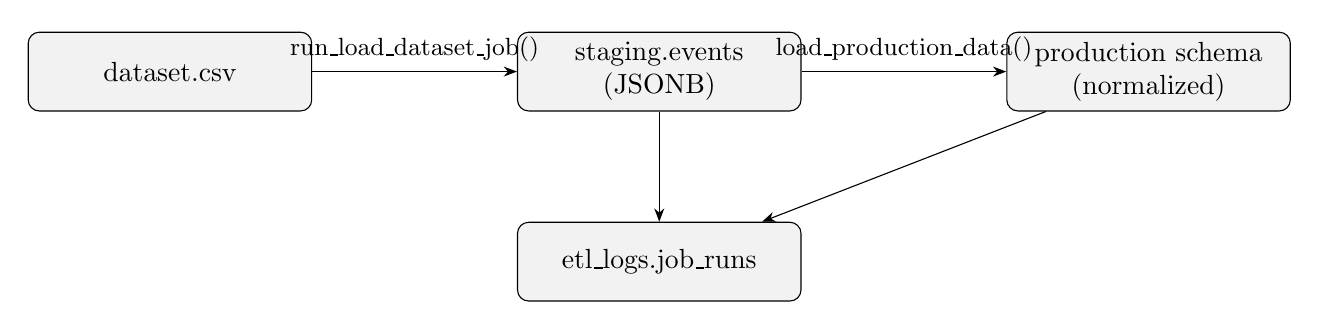
\begin{tikzpicture}[node distance=2.6cm, >=Stealth]
\tikzstyle{box}=[draw, rounded corners, align=center, minimum width=3.6cm, minimum height=1cm, fill=gray!10]
\node[box] (csv) {dataset.csv};
\node[box, right=of csv] (stg) {staging.events\\(JSONB)};
\node[box, right=of stg] (prod) {production schema\\(normalized)};
\node[box, below=1.4cm of stg] (log) {etl\_logs.job\_runs};

\draw[->] (csv) -- node[above]{\small run\_load\_dataset\_job()} (stg);
\draw[->] (stg) -- node[above]{\small load\_production\_data()} (prod);
\draw[->] (stg) -- (log);
\draw[->] (prod) -- (log);
\end{tikzpicture}
\end{center}

\section{Schemas}
\subsection*{Staging}
\textbf{\texttt{staging.events}}(\texttt{stagEventId SERIAL PK}, \texttt{content JSONB}, \texttt{load\_date TIMESTAMP}).\\
Raw rows are stored as JSONB for flexible ingestion. Upserts compare existing \texttt{content} by \texttt{student\_id} and replace on change.

\subsection*{ETL Logging}
\textbf{\texttt{etl\_logs.job\_runs}}(\texttt{logId PK}, \texttt{jobname}, \texttt{status}, \texttt{error\_message}, \texttt{start\_date}, \texttt{end\_date}, \texttt{records\_count}).\\
Helper functions: \texttt{return\_max\_date()}, \texttt{update\_job\_run()}, \texttt{update\_job\_skipped()}, \texttt{update\_job\_failed()} track lifecycle and counts.

\subsection*{Production (Normalized)}
\begin{itemize}[leftmargin=1.2em]
  \item \textbf{\texttt{production.student}}(\texttt{student\_id PK}, \texttt{age}, \texttt{gender})
  \item \textbf{\texttt{production.academic\_performance}}(\texttt{student\_id PK, FK}, GPA/SAT/Field)
  \item \textbf{\texttt{production.skills\_extracurriculars}}(\texttt{student\_id PK, FK}, internships/projects/certifications/soft \& networking scores)
  \item \textbf{\texttt{production.career\_outcomes}}(\texttt{student\_id PK, FK}, offers/salary/satisfaction/promotion/job level/WLB/entrepreneurship)
\end{itemize}
All FKs cascade on delete from \texttt{student}. CHECK constraints enforce domain validity.

\section{Normalization (1NF, 2NF, 3NF)}
\textbf{1NF.} Atomic columns, no repeating groups. JSON is only in staging; production is scalarized per attribute.\\
\textbf{2NF.} All non-key attributes depend on the whole key. Every table uses the simple key \texttt{student\_id}, avoiding partial dependencies.\\
\textbf{3NF.} No transitive dependencies: demographics, academics, skills, and career outcomes are factored into separate tables; each non-key attribute describes the table's subject (no attribute depends on another non-key attribute).

\section{ETL Implementation Details}
\subsection*{Staging Loader (change-aware upsert)}
\textbf{Function:} \texttt{run\_load\_dataset\_job()}\\
\textbf{Logic:} compares \texttt{pg\_stat\_file('.../dataset.csv').modification} with the MAX(\texttt{end\_date}) for job ``dataset-load''. If newer, calls \texttt{upsert\_dataset()}, which bulk loads into a temp table via \texttt{COPY}, then:
\begin{itemize}[leftmargin=1.2em]
  \item \emph{UPDATE} existing \texttt{staging.events} rows where content differs.
  \item \emph{INSERT} missing \texttt{student\_id}s.
\end{itemize}
This is idempotent and minimizes churn.

\subsection*{Production Loader (idempotent upsert)}
\textbf{Function:} \texttt{load\_production\_data()} performs four \texttt{INSERT \ldots ON CONFLICT DO UPDATE} statements from \texttt{staging.events} into normalized tables, preserving keys and enforcing constraints.

\section{Automation (Scheduling with \texttt{pg\_cron})}
\textbf{Extensions/config:} Install \texttt{postgresql-16-cron}; set in \texttt{postgresql.conf}:\\
\texttt{shared\_preload\_libraries='pg\_cron'} and \texttt{cron.database\_name='test\_db'}.\\
\textbf{Jobs:}
\begin{itemize}[leftmargin=1.2em]
  \item \texttt{load-dataset}: every minute — \texttt{SELECT run\_load\_dataset\_job();}
  \item \texttt{etl-job}: every two minutes — \texttt{SELECT load\_production\_data();}
\end{itemize}
These are created via \texttt{SELECT cron.schedule(\ldots)} in the SQL scripts.

\section{Deployment \& Reproducibility}
\subsection*{Docker Image}
\textbf{Dockerfile highlights:}
\begin{itemize}[leftmargin=1.2em]
  \item Base: \texttt{postgres:16}; installs \texttt{postgresql-16-cron}.
  \item Enables \texttt{pg\_cron} via \texttt{shared\_preload\_libraries} and sets \texttt{cron.database\_name}.
  \item Copies \texttt{dataset.csv} and all SQL init scripts into \texttt{/docker-entrypoint-initdb.d/}.
\end{itemize}

\subsection*{Build \& Run}
\begin{enumerate}[leftmargin=1.5em]
  \item Build: \texttt{docker build -t dbd-pipeline .}
  \item Run: \texttt{docker run --name dbd-pg -p 5432:5432 -e POSTGRES\_PASSWORD=postgres dbd-pipeline}
  \item Connect: \texttt{psql -h localhost -U postgres -d test\_db}
\end{enumerate}
The init scripts create schemas, tables, functions, and schedule \texttt{pg\_cron} jobs automatically on first boot.

\section{Logging \& Monitoring}
\texttt{etl\_logs.job\_runs} captures: job name, status, timestamps, error message, and processed record counts. Helper functions consistently transition statuses from \emph{running} to terminal states. Use:
\begin{lstlisting}[language=SQL]
SELECT * FROM etl_logs.job_runs ORDER BY logId DESC LIMIT 20;
\end{lstlisting}

\section{Analysis: Issues \& Improvements (Requirement \#7)}
\subsection*{What works well}
\begin{itemize}[leftmargin=1.2em]
  \item \textbf{Idempotent ETL:} Upserts in both staging and production prevent duplicates and safely re-run jobs.
  \item \textbf{Change-aware ingestion:} Skips loads when the CSV file is unchanged, reducing unnecessary writes.
  \item \textbf{Normalization:} Clear separation of concerns across four production tables with CHECK constraints.
  \item \textbf{Automation:} Fully scheduled via \texttt{pg\_cron} at container start.
\end{itemize}

\subsection*{Limitations Observed}
\begin{itemize}[leftmargin=1.2em]
  \item \textbf{CSV coupling / pathing:} The file is baked into the image at \texttt{/app/dataset.csv}; changing data requires rebuilding or mounting a volume.
  \item \textbf{Atomicity:} Staging and production loads are separate jobs; mid-run failures could leave a mismatch for a short window.
  \item \textbf{Validation at staging:} Staging accepts any JSON shape; malformed rows are only caught when casting to production types.
\end{itemize}

\subsection*{Improvements (Future Work)}
\begin{itemize}[leftmargin=1.2em]
  \item \textbf{Mount dataset as a volume} instead of copying into the image; add checksum-based (SHA256) change detection.
  \item \textbf{Wrap production load in a transaction} and/or use a \emph{swap table} pattern to ensure all-or-nothing refresh.
  \item \textbf{JSON schema validation in staging} (e.g., via \texttt{CHECK (content ? 'student\_id' \&\& (content->>'age')::INT > 0)} or PL/pgSQL validation) to fail fast.
  \item \textbf{Indexes for performance:} \texttt{CREATE UNIQUE INDEX ON staging.events ((content->>'student\_id'));} plus indexes on FK columns in production tables.
  \item \textbf{Observability:} Add metrics tables for per-table row deltas; extend \texttt{job\_runs} with duration milliseconds and more granular error codes.
  \item \textbf{Security:} Create a dedicated role for ETL with least privilege; avoid superuser for runtime jobs.
  \item \textbf{Scheduling cadence:} Switch to daily at 02:00 for production to match a conventional batch window.
\end{itemize}

\section*{Appendix A: File Map}
\begin{longtable}{>{\ttfamily}p{0.36\linewidth}p{0.56\linewidth}}
\toprule
01\_database\_setup.sql & Create DB, schemas (\texttt{staging, production, etl\_logs}), enable extensions.\\
02\_staging\_schema.sql & Staging table, job log table, staging loader \& helper functions, cron job for ingestion.\\
03\_production\_schema.sql & Production tables with constraints, production loader function, cron job for ETL.\\
Dockerfile & PostgreSQL 16 + pg\_cron; copies dataset and init scripts; sets preload libraries.\\
install.sh & Convenience script to install Docker and Compose on Ubuntu.\\
\bottomrule
\end{longtable}

\section*{Compilation Notes}
This document uses standard \LaTeX{} packages. Compile with \texttt{latexmk -pdf DBD\_Documentation.tex}. If you see a ``rerun'' notice, compile a second time to refresh bookmarks/outlines.

\end{document}
